\documentclass{report}
\usepackage{fancyhdr} % Required for custom headers
\usepackage{lastpage} % Required to determine the last page for the footer
\usepackage{extramarks} % Required for headers and footers
\usepackage{graphicx} % Required to insert images
%\usepackage{lipsum} % Used for inserting dummy 'Lorem ipsum' text into the template
\usepackage{amsmath}
\usepackage{graphicx} 
\usepackage{float}
%\usepackage{amsfont}
%\usepackage{amssymb}

\usepackage{multicol}
% Margins
\topmargin=-0.5in
\evensidemargin=0in
\oddsidemargin=-0.5in
\textwidth=7.5in
\textheight=9.0in
\headsep=0.25in 


\pagestyle{fancy}

%\rhead{\textbf{Marshall's Recipes}} % Top right header
%\lhead{\textbf{Curry Stir Fry}}
%\chead{ }
%\title{Curry Stir Fry}

\begin{document}
%\vspace{8mm}
%\textbf{PRELIMINARIES:}


\bigskip

\bigskip

\begin{multicols}{2}
\textbf{Ingredients}
\begin{itemize}


\item 6  onions \quad (270 kCal / 6 gP / 0 gF / 66 gC)
\item 1 lb lentils \quad (1690 kCal / 104 gP / 14 gF / 286 gC)
\item 1 cup of rice \quad (640 kCal / 12 gP / 0 gF / 144 gC)
\item 4 tbsp. olive oil \quad (476 kCal / 0 gP / 56 gF / 0 gC)
\item 12 eggs \quad (936 kCal / 72 gP / 60 gF / 12 gC)
\item 1 tsp salt 
\item 1 tsp cumin 



\end{itemize}


\columnbreak
\textbf{Procedure:}
\medskip


\begin{enumerate}
\item Chop 5 onions. Slice the remaining onion and put in a separate bowl. 
\medskip 
\item Rinse lentils, strain and place in a large pot with 5 cups of water. Bring mixture to a boil, simmer and cook covered until the lentils are tender but not fully cooked, about 15 minutes. Most of the liquid should be absorbed.
\medskip \item While the lentils cook, in a separate large pan, heat two tablespoons of olive oil on medium heat and fry the chopped onions until golden brown, about 10-15 minutes. Remove onions from pan and place in large bowl. Add sliced onion to pan with 2 tbsp. olive oil and on medium heat, fry the sliced onions until golden brown and caramelized - about 15 minutes. In the last couple minutes of frying the onions, you can turn up the heat to high to get a crispy texture.

%Transfer on top of the lentils and rice mixture, add cumin and toss to combine.

\item While sliced onions cook, rinse the rice and transfer to the pot of lentils and season with salt. Add 2 cups water, bring to a boil, then reduce to a simmer and cook covered until the rice is tender, about 18 minutes. Remove the pot from the heat. Allow the rice to rest in the pot for about 5 minutes, without opening the lid, to absorb all the liquid and steam.

\item When onions are nearly done cooking, start frying the eggs in a large pan. While the eggs cook (2 per serving), combine all the onions with the lentil and rice mixture. When the eggs are slightly runny, serve on top of everything with a pinch of salt and pepper. 

 



\begin{table}[H]
  \begin{center}
    \caption{Macro totals}
    \label{tab:table1}
    \begin{tabular}{c|c|c|c} % <-- Alignments: 1st column left, 2nd middle and 3rd right, with vertical lines in between
      \textbf{Calories} & \textbf{Protein} & \textbf{Fat} & \textbf{Carbs}\\
      \hline
      4012 kCal & 194 g & 130 g & 508 g\\
    \end{tabular}
  \end{center}
\end{table}
 
\end{enumerate}
\end{multicols}




%\begin{center}
%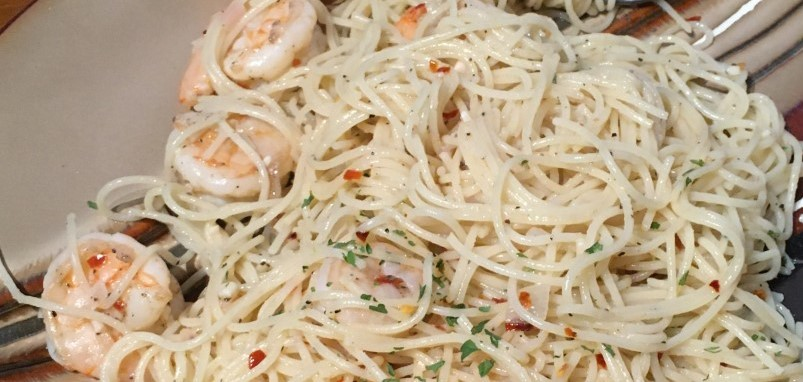
\includegraphics[scale=0.65]{Pasta/Shrimp Scampi/Shrimp Scampi.jpg}
%\end{center}


\end{document}